\documentclass[11pt,a4paper]{report}
\usepackage[margin=1in]{geometry}
\usepackage[T1]{fontenc}
\usepackage{lmodern}
\usepackage{hyperref}
\usepackage{booktabs}
\usepackage{longtable}
\usepackage{listings}
\usepackage{xcolor}
\usepackage{graphicx}
\usepackage{tikz}
\usetikzlibrary{shapes,arrows.meta,positioning}

\hypersetup{colorlinks=true,linkcolor=blue,urlcolor=blue}
\lstdefinestyle{bash}{
  basicstyle=\ttfamily\small,
  breaklines=true,
  frame=single,
  backgroundcolor=\color{gray!8}
}
\lstdefinestyle{proto}{
  basicstyle=\ttfamily\small,
  breaklines=true,
  frame=single,
  backgroundcolor=\color{gray!8}
}

\title{CXR gRPC Lab Manual\\
\large SW.16 --- ClaimAnalysis internal RPC + grpcui}
\author{CXR Ops Lab --- \texttt{cxr-ops-lab}}
\date{2026-05-31}

\begin{document}
\maketitle
\begin{abstract}
\textbf{SW.16}: \texttt{cxr.v1.ClaimAnalysis} gRPC service on \textbf{:50051} with
\texttt{GetClaimStatus} and \texttt{AnalyzeClaim}. Browser UI via \textbf{grpcui :8090}.
Standalone lab --- \textbf{Claim Studio (:3000)} keeps REST + Python \texttt{spawn}.
\end{abstract}
\tableofcontents
\newpage

\chapter{Architecture}

\begin{center}
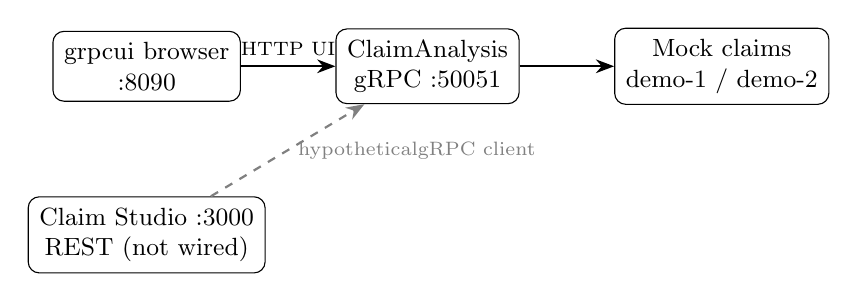
\begin{tikzpicture}[
  node distance=0.65cm and 0.5cm,
  box/.style={draw, rounded corners, minimum height=0.75cm, align=center, font=\small, inner sep=4pt},
  arr/.style={-{Stealth}, thick}
]
  \node[box] (ui) {grpcui browser\\:8090};
  \node[box, right=1.2cm of ui] (grpc) {ClaimAnalysis\\gRPC :50051};
  \node[box, right=1.2cm of grpc] (mock) {Mock claims\\demo-1 / demo-2};
  \node[box, below=1.2cm of ui] (cxr) {Claim Studio :3000\\REST (not wired)};
  \draw[arr] (ui) -- node[above,font=\scriptsize]{HTTP UI} (grpc);
  \draw[arr] (grpc) -- (mock);
  \draw[arr, dashed, gray] (cxr) -- node[right,font=\scriptsize]{hypothetical\\gRPC client} (grpc);
\end{tikzpicture}
\end{center}

\chapter{CXR placement (syllabus M2.8)}

\begin{center}
\begin{tabular}{ll}
\toprule
Today (bootcamp) & Hypothetical gRPC boundary \\
\midrule
UI $\rightarrow$ REST $\rightarrow$ \texttt{spawn} Python & BFF $\rightarrow$ \texttt{AnalyzeClaim} $\rightarrow$ analysis kernel \\
GraphQL :4000 = external query API & gRPC = \textbf{internal} service-to-service \\
Kafka :9092 = async events & Publish \emph{after} analyze; does not replace sync RPC \\
\bottomrule
\end{tabular}
\end{center}

\chapter{Procedure}

\begin{lstlisting}[style=bash]
cd cxr-ops-lab
./scripts/19-grpc-up.sh
./scripts/19-grpc-smoke.sh
\end{lstlisting}

Browser: \textbf{http://localhost:8090} $\rightarrow$ \texttt{cxr.v1.ClaimAnalysis} $\rightarrow$
\textbf{AnalyzeClaim} with \texttt{lab/grpc/request-golden.json}.

\chapter{Proto (golden RPCs)}

\begin{lstlisting}[style=proto]
service ClaimAnalysis {
  rpc GetClaimStatus(GetClaimStatusRequest) returns (ClaimStatusResponse);
  rpc AnalyzeClaim(AnalyzeClaimRequest) returns (AnalyzeClaimResponse);
}
\end{lstlisting}

Golden: \texttt{claim\_id = "demo-1"} $\rightarrow$ \texttt{status = "ok"} (matches SW.15 GraphQL / SW.13 Kafka fixture).

\chapter{Files}

\begin{longtable}{@{}p{5cm}p{8cm}@{}}
\toprule
File & Purpose \\
\midrule
\endhead
\texttt{lab/grpc/cxr\_claim.proto} & Service definition \\
\texttt{lab/grpc/server.mjs} & Node \texttt{@grpc/grpc-js} server \\
\texttt{lab/grpc/client-smoke.mjs} & Healthcheck + smoke client \\
\texttt{compose.grpc.yaml} & Server + grpcui \\
\texttt{scripts/19-grpc-up.sh} & Start stack \\
\texttt{scripts/19-grpc-smoke.sh} & Verify :8090 + RPC \\
\texttt{evidence/SW16-grpc-verify-2026-05-31.md} & Checklist \\
\bottomrule
\end{longtable}

\chapter{Live adjustments}

\begin{itemize}
  \item \textbf{gRPC reflection} --- grpcui requires reflection; \texttt{@grpc/reflection} added to \texttt{server.mjs} (without it grpc-ui container crash-loops).
  \item \textbf{Healthcheck} --- in-container \texttt{client-smoke.mjs} (gRPC has no browser GET on :50051).
  \item \textbf{grpc-ui restart} --- \texttt{19-grpc-up.sh} restarts grpc-ui after server healthy (avoids stale crash-loop from pre-reflection boot).
\end{itemize}

\chapter{UI evidence --- grpcui (:8090)}

\textbf{AnalyzeClaim} form for \texttt{cxr.v1.ClaimAnalysis}. Golden invoke:
\texttt{claim\_id = demo-1}, \texttt{content = SW.16 golden-path fixture}
$\rightarrow$ Response \texttt{status: ok}.

\begin{figure}[htbp]
\centering
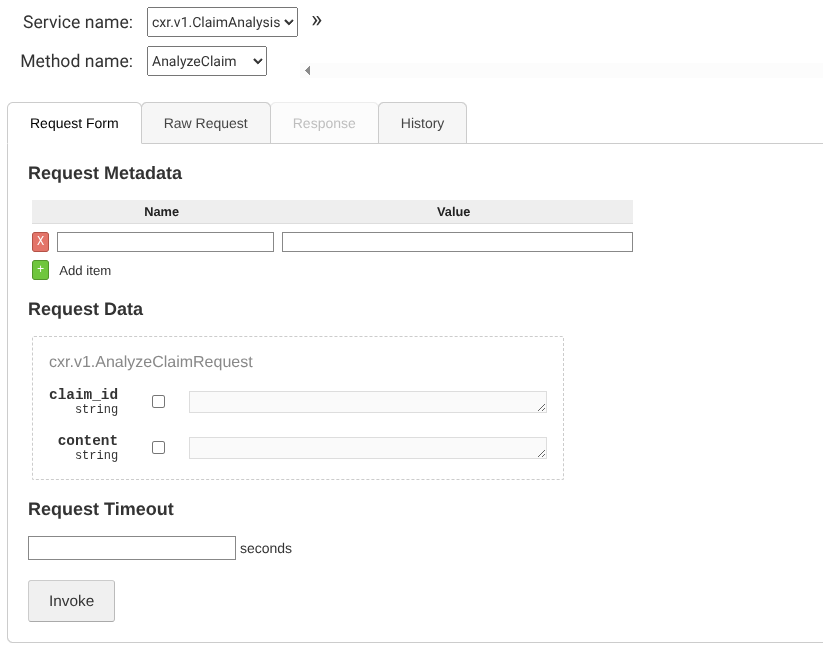
\includegraphics[width=0.92\textwidth]{../evidence/SW16-grpcui-2026-05-31.png}
\caption{grpcui Request Form --- \texttt{AnalyzeClaim} on \textbf{:8090} (user verify 2026-05-31).}
\end{figure}

\chapter{Stop}

\begin{lstlisting}[style=bash]
docker compose -f compose.grpc.yaml down
\end{lstlisting}

\end{document}
